\section{Evaluating the Success of the Project}

Project success depends highly upon perspective, one stakeholder might consider the project beyond successful whereas another stakeholder may consider the project a total failure. Evaluating success must consider a variety of perspectives, and even then it may not be as simple as a yes or no answer. 

\begin{quote}
``An architect may consider success in terms of aesthetic appearance, an engineer in terms of technical competence, an accountant in terms of dollars spent under budget, a human resources manager in terms of employee satisfaction, and chief executive officers rate their success in the stock market.''
%todo reference Freeman and Beale (1992,p. 8) 
\end{quote}

%todo: this is vics stuff, didn't even proof it, shot-not (Laith),
\paragraph{Shenhar et al, 1997} \cite{shenhar} In this paper it is suggested that the traditional measures of project success --- namely time cost and quality --- are perhaps not the best, and points out the disagreement in the literature on this area. Building on evidence from previous studies, the authors suggest a new, multidimensional, framework for project success; and, notably, back this up and expand upon it by utilising empirical evidence.

This evidence takes the form of 127 structured questionnaires, returned from project managers from a variety of industries.\sidenote[][-6em]{It is claimed in the paper that despite this selection having not been made at random, with no consideration to stratification, and that 'the end products were aimed at a military market', that there is not an inherent bias. Especially in light of the low sample size this should be considered to be a somewhat dubious claim.} This data was then analysed using numerical measures from previous work\sidenote[][1em]{Specifically Cooper and Kleinschmidt, 1987;  Pinto and Stevin, 1988; Stuckenbruck, 1986; and Dvir and Shenhar 1992. (See full bibliography).} and the dimensionality of results determined using factor analysis.\sidenote[][1em]{Factor analysis being a statistical technique to determine the underlying dimensionality of a data set without previous knowledge of it. See Brayant and Yarnold (detail in bibliography) for a full treatment.}

Despite an initial hypothesis of three dimensions to project success, the analysis suggests that there are in fact four. These dimensions were then correlated(using Pearson's Correlation) with the overall assessment of project success, with favourable results; and the relative strength of each measured, both for projects in progress and completed projects. The strength was seen to be consistent, apart from the fourth dimension which was significantly better correlated in completed projects. This is the 'future potential' dimension. 

This empirical experiment causes this research to stand out in a way other papers on the subject of project success do not, in that the claims are in fact backed up. This is in sharp contrast to Atkinson's paper (see below).

Another notable feature of this paper is that in addition to the scientific numerical approach, a significant percentage of the text is given to practical consequences of the results and implications for the practitioner. Given that it is now nearly fifteen years old it is surprising that these ideas do not feature more prominently in project management canon.

%%%%%%%%%%%%%%%%%%%%

\paragraph{\textit{Atkinson, 1999} }\cite{atkinson1999} In this dramatically titled\sidenote[][1em]{And somewhat imprecisely titled --- he might have preferred: \emph{Time, cost, and quality in project management: two best guesses and a phenomenon; it's time to accept other success criteria}. } paper, Atkinson attempts to firmly disabuse faith in the so-called `Iron Triangle' of time, cost, and quality as a definitive measure of project success; and instead proposes his own, which he cheerily dubs `The Square Route'.

Atkinson opens with a fairly comprehensive review the of then current literature, but does not seem to use this to great advantage in supporting his own ideas. He frequently annotates his discussion with a distinction between Type I and Type II errors\sidenote[][1em]{The best way of informally defining the distinction between Type I and Type II errors is to think of the former as a \emph{false positive}, and the latter as a \emph{false negative}. Atkinson's definitions are vague and in places misleading.} again without a clear motive. His suggested framework --- the `Square Route' --- does not suggest an obvious way of working to the manager and seems in at least one way to be overly specific: in placing the concept of `the information system' as a pillar of the framework. While this and related concepts may be relevant for many projects, there will be still others that they are not --- hardly a basis for a universal system.

%%%%%%%%%%%%%%%%%%%%

%
%In the paper ``Project management: cost, time and quality, two best guesses and a phenomenon, its time to accept other success criteria'' %todo citation
%, Atkinson considers typical assessment criteria to be insufficient, and proposes a new method known as "The Iron Triangle" which aggregates many existing paradigms to form a new way of evaluating project success.
%
%In the paper ``Mapping the dimensions of project success'' Shenhar et. al. identify four dimensions which measure the success of a project, and can be further used to quantify the success of a project against a benchmark of well known projects throughout history.
%


The Iron Triangle is a primitive tool for measuring the balance between time, cost and quality. It has no quantifiable properties and is mainly an illustrative tool, but it does somewhat accurately express the relation between the three constraints.
\begin{marginfigure}
	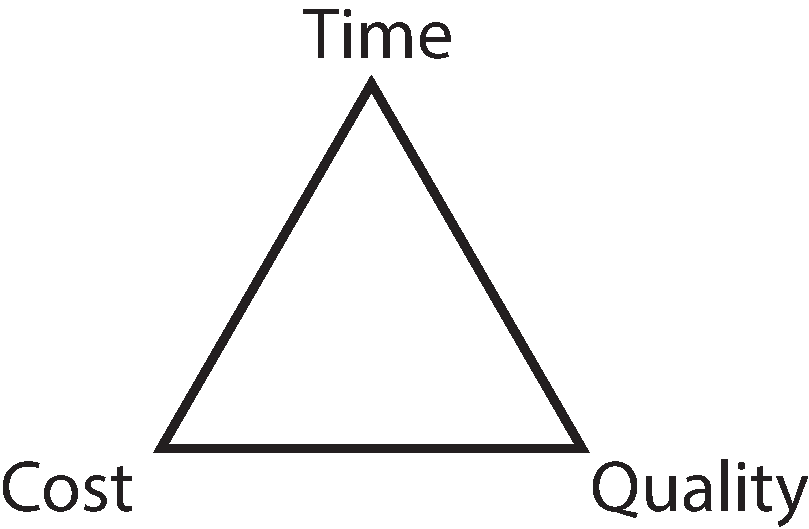
\includegraphics[width=55mm]{res/pm/TCQ_triangle}
	\label{fig:TCQ_triangle}
	\caption{The Iron Triangle}
\end{marginfigure}
Selecting two of the properties as desirable will be costly to the third, for example demanding a high quality product in little time will escalate the cost. The project had no real notion of monetary cost, so the balance was largely between quality, project time and personal time, where the personal cost a team members marks from other assignments, time for hobbies, sleep, etc. For almost all project components there would be an imbalance between the three properties, and most often, the \emph{personal time} property would need to be increased to ensure good quality products while keeping to schedule.  


\paragraph{Success Dimension 1 : Project Efficiency}
The first dimension is interesting in the way it applies to software projects, since efficiency is extremely difficult to guage. Unlike a task requiring manual labour, efficiency can be assessed fairly easily since most tasks are repeatable and hence can be modelled fairly easily. It's difficult, on the other hand, to compare two software projects, since not only are they very rarely alike, but efficiency is not easily quantifiable. Some managers try to quantify development progress by measuring lines of code per day, as Hertzfeld implied in his article ``-2000 lines of code'', the number of lines a developer has written per day may have no bearing on the work accomplished. Even it there was a convenient function of project progress to mark efficiency, that efficiency would likely be subject to changes. Suppose a large software project launches, stays on schedule and outputs an excellent number of lines per day, it might be the case that the developers are taking shortcuts and not being prudent, which could cause a massive slump in the efficiency late down the line when it's discovered that the initial few milestones are bug ridden and need to be revised. By contrast a project team missing the initial deadlines might be investing a large amount of thought into their work which could accelerate their efficiency later down the line. The important thing to note is that efficiency hinges on perspective, and it's very difficult to find a function to assess the efficiency of a software project.
%%todo: Sounds sloppy so far, revise!
Given that it is in fact necessary for the model, it would be wisest to measure efficiency by comparing each estimated milestone completion date with it's actual completion date, since the milestones were all met on time, but some features were lacking, it's fair to claim the project progress was reasonably efficient \emph{efficiency} available. 

\paragraph{Success Dimension 2 : Impact on customer}
%todo: Matt's feedback?

\paragraph{Success Dimension 3 : Business and Direct Success}
Business and Direct success is a measure of whether the project provided ``the sales, income, and profits as expected'', ``increase[d] business results'' or whether the project ``helped to increase market share'' \cite{shenhar}. Shenhar does elaborate that other projects may not fall under the same assessment criteria, but will have some mechanism of measuring direct success. Since this project is academically motivated rather than monetarily driven, it would be fair to assess the success outcomes the requirements discussed in section \ref{sec:reviewrequirements}. The project met most of these requirements, and the requirements it failed to meet were considered the least important. The project was largely successful in creating a fun game in Haskell, which met almost all the functional requirements and fulfilled all the non-functional requirements, granting the project at least a partial success under Dimension 3.
 
\paragraph{Success Dimension 4 : Preparing for the Future}
The fourth dimension investigates how prudent the project is, whether it has invested in future opportunities, whether it explored further ideas, innovations or skills which may be required in the future. Assessment under this dimension can only result in an overwhelming success. The project explored two concepts which are already hugely popular and only growing in popularity, namely indie games and the Haskell programming language. Haskell's growing popularity is undeniable, it's a concise yet extremely powerful language which has recently being adopted by an increasing number of companies including ABN AMRO, Anygma, Amgen, Bluespec and Eaton. It has been used to construct many large scale projects such as ASIC, FPGA (design software), Haskore, GHC, Darcs and HAppS, projects which are of comparable size and complexity of many corporately produced games. \cite{realworldhaskell}

%todo: Probably won't be able to phrase of cite this bit properly tonight
Game development is also a very rapidly growing market, with the advent of mobile devices the target audience for video games barely excludes any social group.  
% Can't think of how to finish this
The project has produced a wealth of experience for developing games in Haskell...

\paragraph{Overall Success}
Each dimension is a measure of success for a time frame, the first being concerned with the immediate results of the project, the fourth being concerned with the distant future and the interactions the project may be a part of in the future. This project was by no means perfect, but it showed strong signs of success when applying Shenhar's success measurement criteria.

